\chapter{Marktanalyse und Relevanz des Projekts}
Die Marktanalyse kommerzieller WordClocks dient der systematischen Untersuchung bestehender Produkte im Hinblick auf technische, funktionale und gestalterische Eigenschaften. 
Ziel ist die Identifikation aktueller Lösungsansätze, technologischer Standards sowie bestehender Einschränkungen. 
Die Analyse bildet eine fundierte Grundlage für die Ableitung eigener Systemanforderungen und unterstützt die Abgrenzung des geplanten Entwicklungsumfangs.

Der Markt für WordClocks lässt sich grundsätzlich in mehrere Segmente unterteilen, die sich hinsichtlich Designanspruch, Funktionsumfang und Preisniveau unterscheiden. 
Im Premiumsegment dominieren Produkte wie die QLOCKTWO EARTH 45 des Herstellers Biegert\&Funk, die primär als Designobjekte positioniert sind. 
Diese Uhren bewegen sich typischerweise in einem Preisbereich von etwa 1.500 € bis über 3.000 €, abhängig von Größe und Materialausführung. 
Sie zeichnen sich durch hochwertige Materialien, minimalistische Gestaltung und eine klare Fokussierung auf die wortbasierte Zeitanzeige aus. 
Erweiterte Funktionen wie Wetterinformationen, Sensorintegration oder kontextbasierte Zusatzinformationen sind in diesem Segment kaum vorhanden~\cite{qlocktwo_earth45}. 
Trotz des hohen Preisniveaus resultiert daraus ein begrenzter funktionaler Mehrwert. Die WordClock von QLOCKTWO in der Ausführung Earth45 Desert ist in Abb.~\ref{fig:qlocktwo_earth45} dargestellt.

\begin{figure}[H]
	\centering
	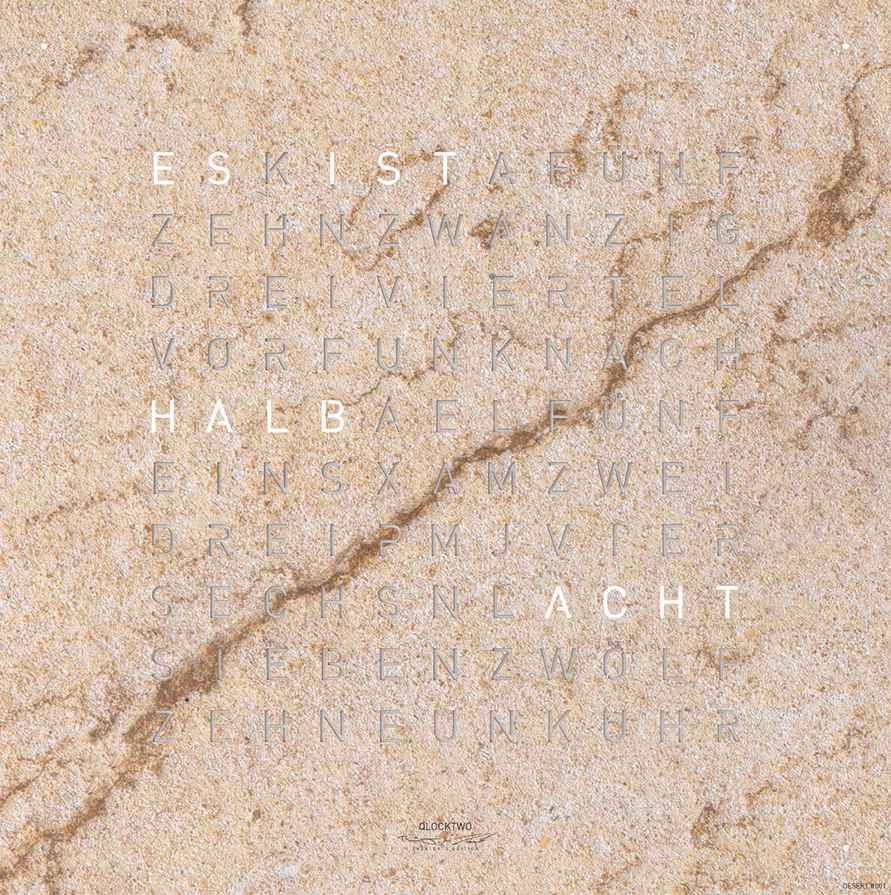
\includegraphics[width=0.45\linewidth]{inhalt/bilder/QlockTwoDessert.png}
	\caption[WordClock Earth45]{Die WordClock Earth45 im Design Desert von QLOCKTWO für einen Kaufpreis von 2.690,00€~\cite{QlockTwoDesertBild}.}
	\label{fig:qlocktwo_earth45}
\end{figure}

Im mittleren Preissegment finden sich technisch erweiterte Lösungen von Herstellern wie Build-Yours oder kleineren Anbietern im Bereich individualisierbarer \gls{led}-WordClocks. 
Ein Beispiel hierfür ist die WordClock Jupiter, die je nach Ausführung in einem Preisbereich von etwa 200 € bis 600 € liegt. 
Diese Systeme erweitern die klassische WordClock um grundlegende Funktionen wie \gls{wlan}-Anbindung, App-Steuerung oder Farbkonfiguration. 
Dadurch wird insbesondere die Individualisierung der Anzeige verbessert. 
Der Funktionsumfang bleibt jedoch überwiegend auf die Darstellung der Uhrzeit sowie visuelle Anpassungen beschränkt, während eine weitergehende Informationsintegration, beispielsweise durch externe Datenquellen, nur eingeschränkt umgesetzt wird~\cite{wordclock_jupiter}.
Eine Ausführung der WordClock Jupiter ist in Abb.~\ref{fig:wordclock_jupiter_stahl} dargestellt.

\begin{figure}[H]
	\centering
	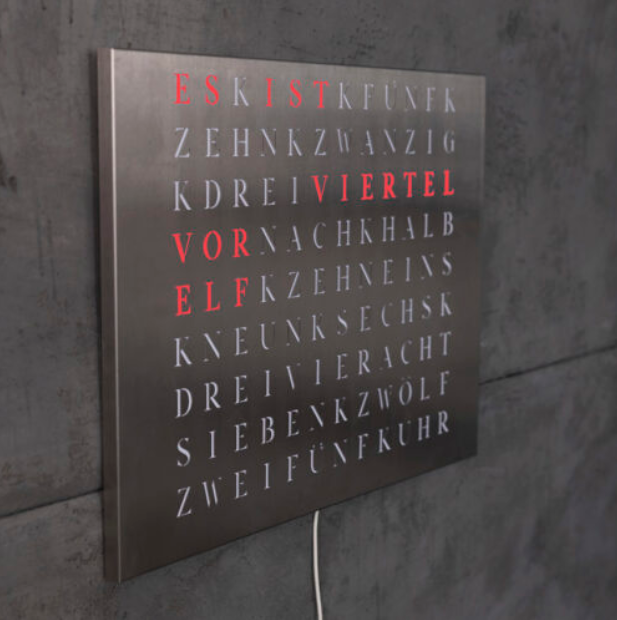
\includegraphics[width=0.3\linewidth]{inhalt/bilder/Jupiterstahl.png}
	\caption[Wordclock Jupiter]{Die Wordclock Jupiter von build-yours.de in Edelstahl gelasert für einen Kaufpreis von 349,00€~\cite{wordclock_jupiter_stahl}.}
	\label{fig:wordclock_jupiter_stahl}
\end{figure}

Ein weiteres Segment bilden günstige Massenmarktprodukte, die über Onlineplattformen wie Alibaba oder vergleichbare Anbieter vertrieben werden. 
Diese Produkte liegen preislich meist im Bereich von etwa 10 € bis 150 € und zeichnen sich durch eine einfache technische Umsetzung sowie eine stark reduzierte Funktionalität aus. 
Sie sind primär als dekorative Produkte einzuordnen und weisen sowohl in Bezug auf Materialqualität als auch Funktionsumfang deutliche Einschränkungen auf~\cite{alibaba_wordclock}.
Ein Beispiel ist in Abb.~\ref{fig:alibaba_wordclock_bild} abgebildet.
\begin{figure}[H]
	\centering
	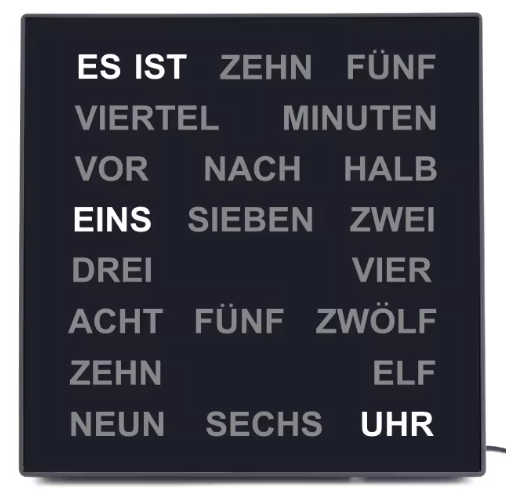
\includegraphics[width=0.3\linewidth]{inhalt/bilder/bildalibaba.png}
	\caption[Beispiel einer Tischwortuhr]{Beispiel einer Tischwortuhr, über Alibaba.com bestellbar zu einem Kaufpreis von weniger als 20~€ bei Abnahme einer entsprechend großen Stückzahl~\cite{alibaba_wordclock_bild}.}
	\label{fig:alibaba_wordclock_bild}
\end{figure}
Zur systematischen Bewertung der betrachteten Systeme werden selbst definierte Kriterien verwendet. 
Die Gegenüberstellung ermöglicht die Identifikation von Gemeinsamkeiten und Unterschieden zwischen den betrachteten Systemen. 
Auf dieser Grundlage lassen sich funktionale Defizite sowie Potenziale für Erweiterungen ableiten. 
Die gewonnenen Erkenntnisse fließen in die Konzeptionierung der im Rahmen dieser Arbeit entwickelten WordClock ein. 
Die definierten Kriterien und Ergebnisse sind in Tabelle~\ref{tab:vergleich_wordclock_ohne_diy} dargestellt.

\begin{table}[H]
\caption[Vergleich verschiedener WordClocks]{Vergleich verschiedener WordClocks in verschiedenen Preissegmenten anhand selbst definierter Kriterien}
\centering
\begin{tabular}{|p{4cm}|p{3.5cm}|p{3.5cm}|p{3.5cm}|}
\hline
\textbf{Kriterium} & \textbf{Premium} & \textbf{Mittleres Segment} & \textbf{Massenmarkt} \\
\hline
Preisbereich & 1.500 € – 3.000 € & 200 € – 600 € & 10 € – 150 € \\
\hline
Zielsetzung & Designobjekt & Technik \& Design & Dekorationsprodukt \\
\hline
Wortbasierte Zeit & Ja & Ja & Ja \\
\hline
Materialqualität & Sehr hoch (Metall, Holz) & Mittel bis hoch & Niedrig \\
\hline
Designfokus & Sehr hoch & Mittel & Gering \\
\hline
WLAN / Internet & Nein & Ja & Nein \\
\hline
App-Steuerung & Nein & Ja & Nein \\
\hline
Anzeigeanpassung & sehr begrenzt & Ja & begrenzt \\
\hline
Sekundenanzeige & Ja (teilweise) & Nein & Nein \\
\hline
Wetterdaten & Nein & Nein & Nein \\
\hline
Temperaturanzeige & Nein & Nein & Nein \\
\hline
Zusatzinfos & Nein & Nein & Nein \\
\hline
Benutzerfreundlichkeit & Sehr hoch & Hoch & Mittel \\
\hline
Produktreife & Sehr hoch & Hoch & Mittel \\
\hline
\end{tabular}
\label{tab:vergleich_wordclock_ohne_diy}
\end{table}

Aus der Gegenüberstellung ergibt sich eine Diskrepanz zwischen Designqualität und funktionaler Leistungsfähigkeit. 
Im Premiumsegment zeigt sich trotz hoher Preise ein eingeschränkter Funktionsumfang.
Bei der QLOCKTWO CLASSIC ist z.B. eine Sekundenanzeige grundsätzlich möglich, erfordert jedoch dass diese durch Drücken eines Knopfes ein- und ausgeschalten wird.
Die Sekundenanzeige erscheint dann als Ziffer durch gezieltes setzen der \gls{led}s auf der Buchstabenmatrix, wodurch die Stundenanzeige unterbrochen ist~\cite{QlockTwoClassicSekundenanzeige}. 
Systeme im mittleren Preissegment bieten erste Ansätze technischer Erweiterungen, erreichen jedoch keine umfassende funktionale Integration moderner Informationssysteme. 
\gls{diy}-Systeme weisen eine hohe Funktionalität und Flexibilität bei vergleichsweise geringen Kosten auf, erfüllen jedoch häufig nicht die gestalterischen und konstruktiven Anforderungen eines marktfähigen Produkts.

Vor diesem Hintergrund gewinnt die Entwicklung einer eigenen WordClock besondere Relevanz. 
Ziel ist es, bestehende Schwächen der aktuellen Marktsegmente gezielt zu adressieren und eine Lösung zu entwickeln, die gestalterische und funktionale Anforderungen integriert. 
Die entwickelte WordClock soll folgenden, grundlegenden und zusätzliche Funktionen aufweisen und darstellen (vgl. Tabelle~\ref{tab:SollFunktionen})

\begin{table}[H]
%\captionsetup{justification=raggedright,singlelinecheck=false}
\caption{Funktionen der entwickelten WordClock}
\centering
\begin{tabular}{cl}
\textbf{Nr.} & \textbf{Grundsätzliche Funktionen} \\ \hline
G1 & Kontinuierliche sprachbasierte Zeitanzeige von Stunde, Minute und Sekunde \\
G2 & Wortbasierte Anzeige der Außentemperatur auf Basis definierter Schwellenwerte \\
G3 & Wortbasierte Darstellung von Wetterinformationen \\
G4 & Symbolische Darstellung der Tageszeit \\
G5 & Symbolische Darstellung der Mondphase \\
G6 & Symbolische Darstellung der Raumfeuchtigkeit \\
G7 & Symbolische Darstellung der Innenraumtemperatur \\
\end{tabular}
\label{tab:SollFunktionen}
\end{table}

Die Bewertung in Tabelle~\ref{tab:bewertung_wordclock} mit einer Skala von 1 (schlecht) bis 5 (sehr gut) zeigt, dass bestehende Systeme entweder in einzelnen Kategorien hohe Ausprägungen erreichen oder deutliche Defizite aufweisen, jedoch keine ausgewogene Gesamtlösung darstellen. 
Premiumprodukte erzielen hohe Werte im Bereich Design und Benutzerfreundlichkeit, weisen jedoch Defizite im Funktionsumfang und der Darstellung von Zusatzinformationen auf. 

\begin{table}[h]
\caption[Bewertung der verschiedenen Preissegmente]{Bewertung der verschiedenen Preissegmente und Definition der angestrebten Werte der entwickelten WordClock}
\centering
\begin{tabular}{|c|c|c|c|c|c|c|}
\hline
\textbf{Produkt} & \textbf{Design} & \textbf{Funktion} & \textbf{Usability} & \textbf{Preis-Leistung} & \textbf{Gesamt} \\
\hline
QLOCKTWO & 5 & 2 & 5 & 2 & 3,5 \\
\hline
Jupiter & 3 & 3 & 4 & 3 & 3,25 \\
\hline
Massenmarkt & 2 & 1 & 3 & 4 & 2,5 \\
\hline
Eigene WordClock & 4 & 5 & 4 & 4 & 4,25 \\
\hline
\end{tabular}
\label{tab:bewertung_wordclock}
\end{table}

Im Rahmen dieser Arbeit wird das Ziel verfolgt, eine WordClock zu entwickeln, die in allen betrachteten Kategorien hohe Bewertungen erreicht, während die Kosten niedrig gehalten werden. 
Hierdurch soll eine ausgewogene und leistungsfähige Gesamtlösung realisiert werden.
Die entwickelte Lösung soll sich zwischen den bestehenden Marktsegmenten positionieren wobei eine bislang nur unzureichend besetzte Nische adressiert wird. 
Sie stellt nicht nur eine technische Erweiterung bestehender Systeme dar, sondern verfolgt den Ansatz, die WordClock von einem Designobjekt zu einem Informationssystem weiterzuentwickeln. 
Die Kombination aus gestalterischer Qualität und funktionaler Erweiterbarkeit begründet die Relevanz der eigenen Entwicklung sowohl aus technischer als auch aus marktbezogener Perspektive.